
\section{New Energy-Aware Scheduling Algorithms} \label{sec:algorithms}
We have developed two new techniques that, when combined with known scheduling algorithms, reduce the likelihood of an energy violation while meeting task deadlines.  We call the algorithms the \emph{Smooth to Average Method} (\textsc{stam}) and \emph{Smooth to Full Utilization} (\textsc{stfu}).

\subsection{Smooth to Average Method}
First we illustrate a core concept, \emph{virtual tasks}, used in our methods.

\begin{definition}
Given a task $\tau_i = <T_i, D_i, P_i>$ and a power threshold value $\bar{P}$, its equivalent \emph{virtual task} is defined as the task $\bar{\tau}_i = <T_i, \bar{D}_i, \bar{P}_i>$.  For \textsc{stam}, $\bar{D}_i = \lceil D_i \times  P_i / \bar{P} \rceil$ and $\bar{P}_i = D_i \times  P_i / \bar{D}_i$.  We use a power threshold $\bar{P} = \sum_i (P_i \times D_i / T_i )$.
\end{definition}

To distinguish, we call the real task $\tau_i$ a \emph{physical task} in the rest of the paper.

\begin{remark}
When the power threshold value $\bar{P}$ is larger than $P_i$, the task $\tau_i$ is the same as the task $\bar{\tau}_i$. When the power threshold value $\bar{P}$ is smaller than $P_i$, task $\tau_i$ and the virtual task $\bar{\tau}_i$ will consume the same amount of energy, but the virtual task $\bar{\tau}_i$ spreads over a longer execution time than task $\tau_i$. Any scheduling algorithm that can schedule the virtual task without violating its deadline constraint will meet the deadline for the physical task as well.
\end{remark}
\begin{remark}
The motivation of introducing virtual tasks is to smooth the energy consumption in the long run. If we make a schedule using the virtual tasks, and then execute the physical tasks according to that schedule, the system will implicitly wait for energy replenishment before running a request that consumes a large amount of energy. The waiting time is proportional to the energy amount consumed by the request.
\end{remark}

Intuitively, it would be a good choice to smooth the energy consumption to the average power requirement of all tasks in a given task list. The \textsc{stam} is designed for such a purpose. We generate a set of equivalent \emph{virtual tasks} by increasing the duration of any task that uses greater than average power, thus \emph{smoothing} each task to approximately the average power. In these virtual tasks, the total energy remains the same as that in the real tasks.  Virtual tasks cannot be scheduled to run at the same time and are not preemptible.  Once the virtual tasks are scheduled, the physical tasks are inserted at the end of the corresponding virtual task's timeslot.  Thus a physical task that consumes high energy is guaranteed to run after an idle period during which energy is harvested, and so the likelihood decreases that the system will run out of energy when the task runs. 

\begin{algorithm}[htb]
\label{stamalg}
\begin{algorithmic}
\STATE INPUT: $realTasks$ \COMMENT {list of [period, duration, power]} 
\STATE INPUT: $N$ \COMMENT {number of tasks}
\STATE OUTPUT: $vTasks$ \COMMENT {same format as $realTasks$}
\STATE $\bar{P} \gets mean(realTasks[:,3])$
\FOR{$i = 1$ \TO $N$}
\IF{$taskList[i,3] > \bar{P}$}
\STATE $E \gets realTasks[i, 2] \times realTasks[i,3]$
\STATE $\bar{D} \gets \lceil E / \bar{P} \rceil$
\STATE $\bar{P} \gets \frac{E}{\bar{D}}$
\STATE $vTasks[i,:] \gets [taskList[i,1]~~\bar{D}~~\bar{P}]$
\ELSE
\STATE $vTasks[i,:] \gets taskList[i,:]$
\ENDIF
\ENDFOR
\end{algorithmic}
\caption{Generate \textsc{stam} Task List}
\end{algorithm}

The \textsc{stam} algorithm calculates the energy consumption of each task by multiplying its runtime by the task's power consumption. After taking the mean energy consumption across all of the tasks in the task list, each task is compared to this value and virtual tasks are generated accordingly. If the given task's power consumption is above the mean power value, the virtual duration is calculated by taking the ceiling of the energy of the task divided by the calculated power mean. This will extend the duration of the virtual task allowing the total energy consumed to be more evenly distributed across the duration of the task's runtime. If the given task's power consumption is below the calculated energy mean, the algorithm is unable to perform any smoothing and will use the unchanged physical task to generate a schedule. The pseudocode of generating \textsc{stam} task list can be found in Algorithm 1.  

\subsection{Smooth to Full Utilization}

A potential problem of \textsc{stam} is that the virtual tasks may be spread across too long a duration, such that no scheduling is possible to meet the virtual tasks' deadline constraints. This may happen if some physical tasks require very high energy and thus the corresponding virtual tasks force the system to wait for a long time. To avoid this problem, we propose a different heuristic to smooth the energy consumption, called \emph{Smooth to Full Utilization} (\textsc{stfu}).  A \emph{virtual task} generated by \textsc{stfu} is defined as the task $\bar{\tau}_i = <T_i, \bar{D}_i, \bar{P}_i>$ where $\bar{D}_i = \lceil D_i \times  P_i / \bar{P} \rceil$ and $\bar{P}_i = D_i \times  P_i / \bar{D}_i$.

The \textsc{stfu} algorithm is similar to \textsc{stam}, but instead of smoothing all tasks to the average energy usage, \textsc{stfu} attempts to create a virtual task list with $100\%$ \emph{virtual utilization}\footnote{The CPU utilization calculated based on virtual tasks is called virtual utilization.}, $U_V$.  In other words, in a schedule generated from a virtual task list output by \textsc{stfu}, the likelihood of there being a virtual task scheduled at any arbitrary time is as close as possible to $100\%$.

Utilization $U$ is defined in equation~\ref{eqn:utilization}, where $k$ is the number of tasks, $D_i$ is the duration of the $i^{th}$ task, and $T_i$ is the period of the $i^{th}$ task.
\begin{equation}
\label{eqn:utilization}
U = \sum_{i=1}^{k} \frac{D_i}{T_i}
\end{equation}

To generate a virtual task list with \textsc{stfu}, first each task is given a virtual duty cycle $d_V$ representing what proportion of the total runtime will be allocated to the corresponding virtual task.  The goal of \textsc{stfu} is to allocate more time to tasks that use greater energy, so that a high-energy task has more time to harvest energy before executing.  For example, a task that uses $40\%$ of the total energy consumed by tasks should be given a virtual duty cycle of $d_V=40\%$.  Virtual tasks cannot have a shorter duration than their real equivalents (otherwise the real task would not fit in the virtual task's timeslice), so if a task's physical duty cycle $d$ is greater than $d_V$ then it will be unchanged. The pseudocode of generating \textsc{stfu} task list could be found in Algorithm 2.

\begin{algorithm}[htb]
\label{alg:stfualg}
\begin{algorithmic}
\STATE INPUT: $realTasks$ \COMMENT {list of $\bar{\tau}_i = <T_i, D_i, P_i>$} 
\STATE INPUT: $N$ \COMMENT {number of tasks}
\STATE OUTPUT: $vTasks$ \COMMENT {same format as $realTasks$}
\STATE $E_{total} = 0$
\FOR{$i = 1$ \TO $N$}
\STATE $d_i \gets D_i / T_i$
\STATE $E_i \gets d_i \times P_i$
\STATE $E_{total} \gets E_{total} +E_i$
\ENDFOR
\FOR{$i = 1$ \TO $N$}
\STATE $d \gets E_i / E_{total}$
\STATE $d_{V} \gets max(D_i, \left \lfloor T_i \times d \right \rfloor)$
\STATE $P_V \gets D_i \times P_i / d_{V}$
\STATE $vTasks[i] \gets [T_i~~d_{V}~~P_V]$
\ENDFOR
\end{algorithmic}
\caption{Generate \textsc{stfu} Task List}
\end{algorithm}

Figure~\ref{fig:edftasksched}, Figure~\ref{fig:stamtaskplot}, and Figure~\ref{fig:stfutaskplot} show four tasks scheduled by \textsc{edf}, \textsc{edf} with \textsc{stam}, and \textsc{edf} with \textsc{stfu}, respectively.  Like in \textsc{stam}, each real task with \textsc{stfu} smoothing is scheduled at the end of its virtual equivalent's time slice.  The third task, which uses the most energy over a long run, is scheduled after a long period spent collecting energy.  The second task uses very little energy overall, and is given just a short period to collect energy.  For this task set, $U \approx 27\%$ and $U_V \approx 96\%$.


\begin{figure}[tb]
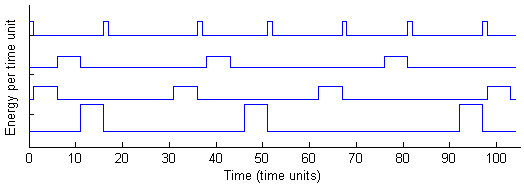
\includegraphics[scale=0.64]{edftasks.png}
\caption{Four tasks scheduled by \textsc{edf} with no smoothing.\label{fig:edftasksched}}
\end{figure}

\begin{figure}[tb]
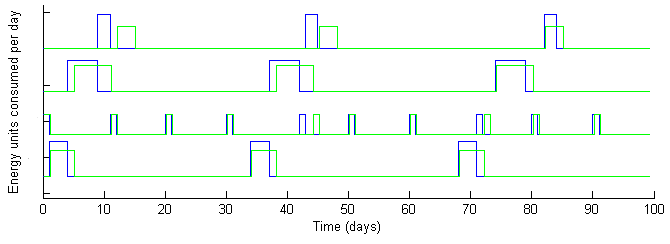
\includegraphics[scale=0.64]{stamtasks.png}
\caption{Four tasks scheduled by \textsc{edf} with \textsc{stam} smoothing.\label{fig:stamtaskplot}}
\end{figure}


\begin{figure}[tb]
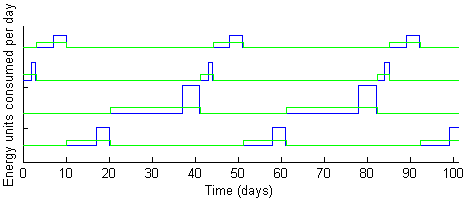
\includegraphics[scale=0.64]{stfutasks.png}
\caption{Four tasks scheduled by \textsc{edf} with \textsc{stfu} smoothing.\label{fig:stfutaskplot}}
\end{figure}



































